% Metódy inžinierskej práce

\documentclass[10pt,twoside,slovak,a4paper]{article}

\usepackage[slovak]{babel}
%\usepackage[T1]{fontenc}
\usepackage[IL2]{fontenc} % lepšia sadzba písmena Ľ než v T1
\usepackage[utf8]{inputenc}
\usepackage{graphicx}
\usepackage{url} % príkaz \url na formátovanie URL
\usepackage{hyperref} % odkazy v texte budú aktívne (pri niektorých triedach dokumentov spôsobuje posun textu)

\usepackage{cite}
%\usepackage{times}

\pagestyle{headings}

\title{Rozvoj e-learningu a stratégie využívané vonline vyučovaní\thanks{Semestrálny projekt v predmete Metódy inžinierskej práce, ak. rok 2020/21, vedenie: Michal Hatala}} % meno a priezvisko vyučujúceho na cvičeniach

\author{Michal Magula\\[2pt]
	{\small Slovenská technická univerzita v Bratislave}\\
	{\small Fakulta informatiky a informačných technológií}\\
	{\small \texttt{...@stuba.sk}}
	}

\date{\small 29. október 2020} % upravte



\begin{document}

\maketitle

\begin{abstract}
	Za posledné roky sa e-learning veľmi spopularizoval. Dôvodom je najmä zlacňovanie osobnej elektroniky
	a výrazné zlepšovanie internetového pokrytia. Hoci týmto systémom je možné sa vzdelávať kedykoľvek
	a kdekoľvek, je stále potrebné vyskúšať mnoho postupov výučby a až časom zistíme, čo je najvhodnejšie.
	Preto účelom tohto článku je oboznámiť čitateľa ohľadom problematiky e-learningu, z čoho e-learning
	vznikol a ako sa vyvinul do podoby v akej ho poznáme dnes. Ďalším cieľom je poskytnúť informácie práve
	ohľadom trendov a stratégií využívaných v online výučbe.
\end{abstract}



\section{Ako sa e-vzdelávanie vyvíjalo}

	Mnoho ľudí si mýli pojem e-vzdelávanie s distančným vzdelávaním a myslia si, že sú tieto slová synonymami.
	V skutočnosti sú to dva rozdielne pojmy. Vývoj e-vzdelávania nastal v 90. tych rokoch spolu s rozvojom internetu.
	Samozrejme nemôžeme poprieť, že e-learning nemá svoje korene v dištančnom vzdelávaní.

	Prvé náznaky dištančného vzdelávania datujeme v roku 1828, keď Profesor C. Phillips inzeroval do novín
	Boston Gazette ponuku na učebné materiály a tutoriály odosielané poštou. V roku 1843 bola 
	založená Phonographic Correspondence Society, ktorá by mohla byť považovaná za prvú inštitúciu 
	venujúcu sa dištančnému vzdelávaniu. Žiaci, ktorí sa zúčastnovali ich kurzu dostávali poštou
	nové a opravené zadania.

	V 20. tych rokoch 20. teho storočia s príchodom masovo komunikačných prostriedkov sa začala formovať aj idea
	vzdelávania žiakov cez tieto prostriedky. Tento nápad bol uskútočnený až v 60. tych tokoch minulého storočia 
	vznikom Open University in UK (Otvorenej univerzity v Spojenom Kráľovstve).



\section{Nejaká časť} \label{nejaka}

Z obr.~\ref{f:rozhod} je všetko jasné. 

\begin{figure*}[tbh]
\centering
%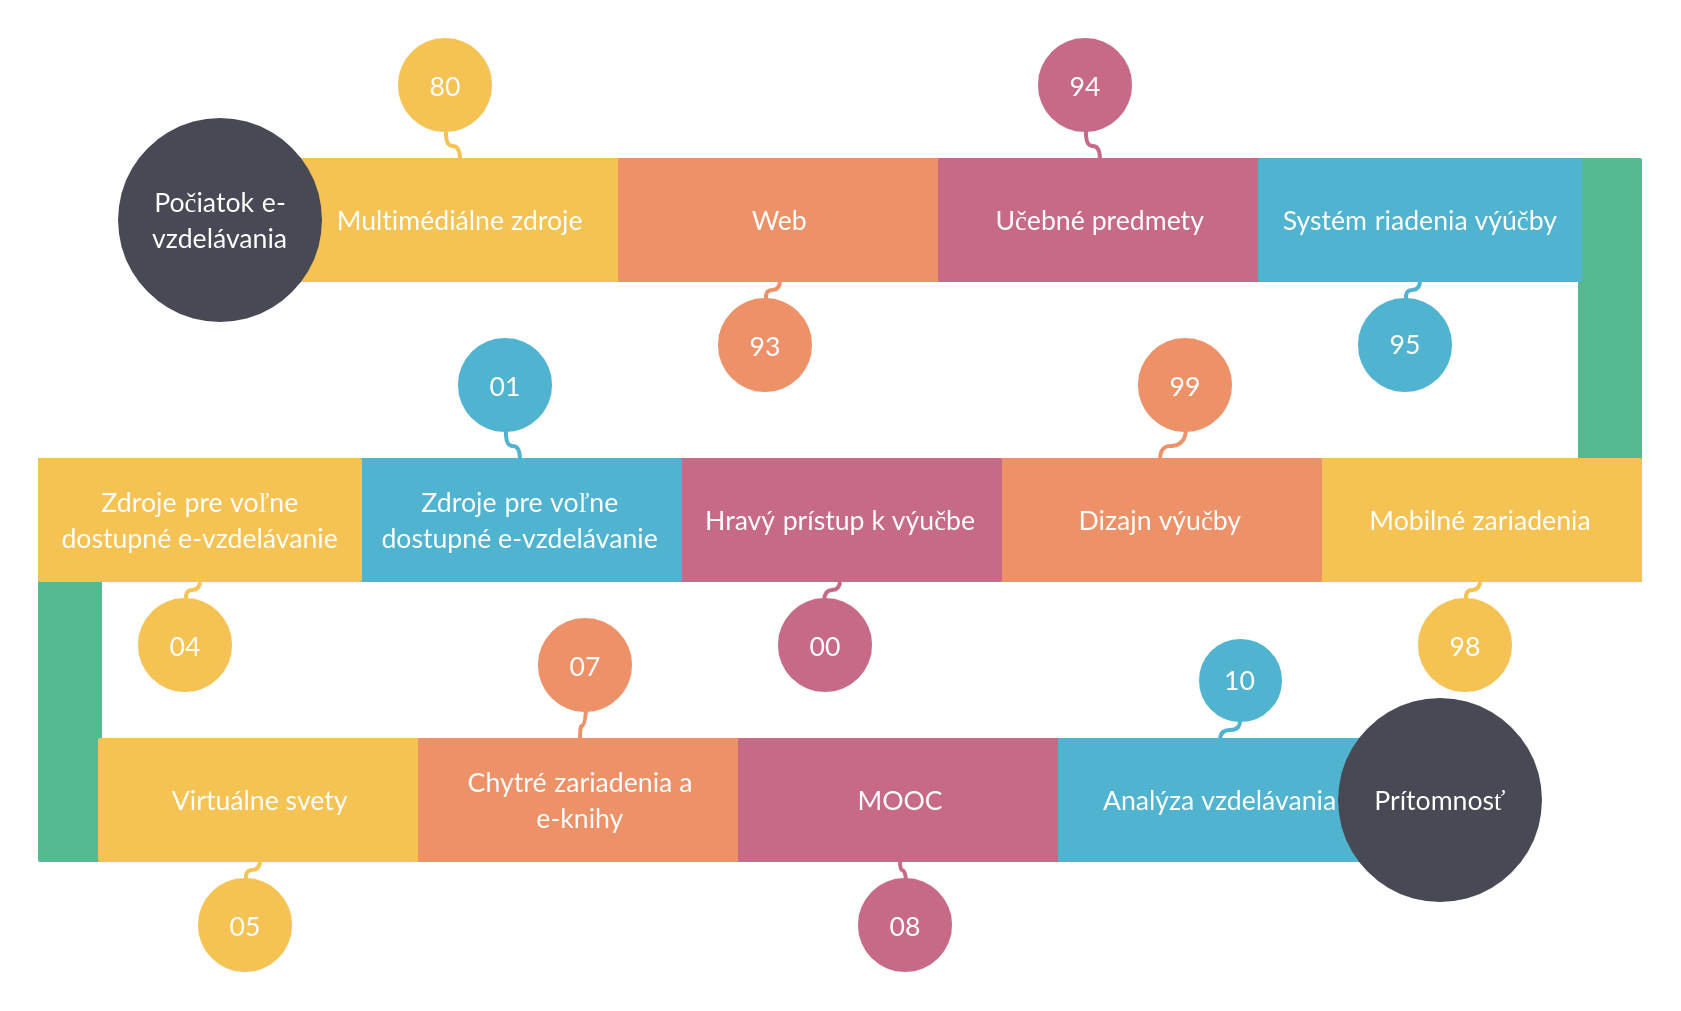
\includegraphics[scale=1.0]{diagram.pdf}
Aj text môže byť prezentovaný ako obrázok. Stane sa z neho označný plávajúci objekt. Po vytvorení diagramu zrušte znak \texttt{\%} pred príkazom \verb|\includegraphics| označte tento riadok ako komentár (tiež pomocou znaku \texttt{\%}).
\caption{Rozhodujúci argument.}
\label{f:rozhod}
\end{figure*}



\section{Iná časť} \label{ina}

Základným problémom je teda\ldots{} Najprv sa pozrieme na nejaké vysvetlenie (časť~\ref{ina:nejake}), a potom na ešte nejaké (časť~\ref{ina:nejake}).\footnote{Niekedy môžete potrebovať aj poznámku pod čiarou.}

Môže sa zdať, že problém vlastne nejestvuje\cite{Coplien:MPD}, ale bolo dokázané, že to tak nie je~\cite{Czarnecki:Staged, Czarnecki:Progress}. Napriek tomu, aj dnes na webe narazíme na všelijaké pochybné názory\cite{PLP-Framework}. Dôležité veci možno \emph{zdôrazniť kurzívou}.


\subsection{Nejaké vysvetlenie} \label{ina:nejake}

Niekedy treba uviesť zoznam:

\begin{itemize}
\item jedna vec
\item druhá vec
	\begin{itemize}
	\item x
	\item y
	\end{itemize}
\end{itemize}

Ten istý zoznam, len číslovaný:

\begin{enumerate}
\item jedna vec
\item druhá vec
	\begin{enumerate}
	\item x
	\item y
	\end{enumerate}
\end{enumerate}


\subsection{Ešte nejaké vysvetlenie} \label{ina:este}

\paragraph{Veľmi dôležitá poznámka.}
Niekedy je potrebné nadpisom označiť odsek. Text pokračuje hneď za nadpisom.



\section{Dôležitá časť} \label{dolezita}




\section{Ešte dôležitejšia časť} \label{dolezitejsia}




\section{Záver} \label{zaver} % prípadne iný variant názvu



%\acknowledgement{Ak niekomu chcete poďakovať\ldots}


% týmto sa generuje zoznam literatúry z obsahu súboru literatura.bib podľa toho, na čo sa v článku odkazujete
\bibliography{literatura}
\bibliographystyle{plain} % prípadne alpha, abbrv alebo hociktorý iný
\end{document}
